\documentclass[10pt,twoside,slovak,a4paper]{article}

\usepackage[slovak]{babel}
\usepackage[IL2]{fontenc}
\usepackage[utf8]{inputenc}
\usepackage{graphicx}
\usepackage{url} % príkaz \url na formátovanie URL
\usepackage{hyperref} % odkazy v texte budú aktívne (pri niektorých triedach dokumentov spôsobuje posun textu)

\usepackage{cite}
%\usepackage{times}

\pagestyle{headings}

\title{3D zváranie, jeho princíp, použitie a perspektíva do budúcnosti\thanks{Semestrálny projekt v predmete Metódy inžinierskej práce, ak. rok 2021/22, 
vedenie: \newline Ing. Vladimír Mlynarovič, PhD.}}

\author{Juraj Marcinech\\[2pt]
	{\small Slovenská technická univerzita v Bratislave}\\
	{\small Fakulta informatiky a informačných technológií}\\
	{\small \texttt{xmarcinech@stuba.sk}}
	}

\date{\small 5. November 2021} 



\begin{document}

\maketitle

\begin{abstract}

Cieľom článku bude zamerať sa na offline programovanie – generovanie pohybového programu robota
prostredníctvom plánovania trajektórie a simulácie pohybu vo virtuálnom prostredí. Postupný
prechod z 2D formátu na 3D - technológiou senzorov a offline programovaním, aby vytvorili
inteligentný navádzací systém zváracieho robota pre 3D zakrivené zvary. Nakoľko súčasný režim
programovania vizuálneho navádzania zvaru je väčšinou 2D vnímanie, ktoré nedokáže priamo
vykonávať presné určovanie polohy a modelovanie zložitých 3D zvarov. Preto je potrebné zvyšovanie
presnosti a zlepšovanie strojového učenia. A je nevyhnutné aby robot mal schopnosť inteligentného
vnímania aby získal potrebné informácie na spracovanie informácií, generovanie programu pohybu a
prevádzku. A v neposlednom rade aj autonómne rozhodovanie medzi typmi zvarov a následne ich
kontrola.

\end{abstract}



\section{Úvod}  %1

% skontroluj si ci si zamenil pojmy OLP a AIsys !!! pripadne prerob i abstrakt troska :)				

V mojom článku by som sa chcel venovať 3D zváraniu, jeho princípu, použitiu a perspektíve do budúcna. 3D zváranie je téma z oblasti strojárstva, ale aj z oblasti modelovania softvérového inžinierstva, nakoľko bez vytvorenia modelov a dôkladnej analýze by bolo nemožné dané problémy vyriešiť.
V posledných rokoch išiel vývoj prudko dopredu, rovnako aj kvalita. Tento proces si ale vyžaduje veľké množstvo schopných programátorov, ktorí vedia kreatívne vyriešiť niekedy naozaj komplikované zvary. Celý tento automatizačný proces je veľmi dôležitý, nakoľko zvyšovaním kvality sa taktiež aj zvyšuje miera bezpečnosti daných produktov a ich trvácnosti.
Perspektívou do budúcnosti je najmä sústredenie sa na vývoj a učenie umelej inteligencie, ktorá bude všetky úlohy vykonávať miesto programátorov a tak sa zredukuje počet chýb na minumum a kvalita bude ešte lepšia.

\section{Myšlienková mapa} \label{mapa} %2

\begin{figure}[htbp]
\centerline{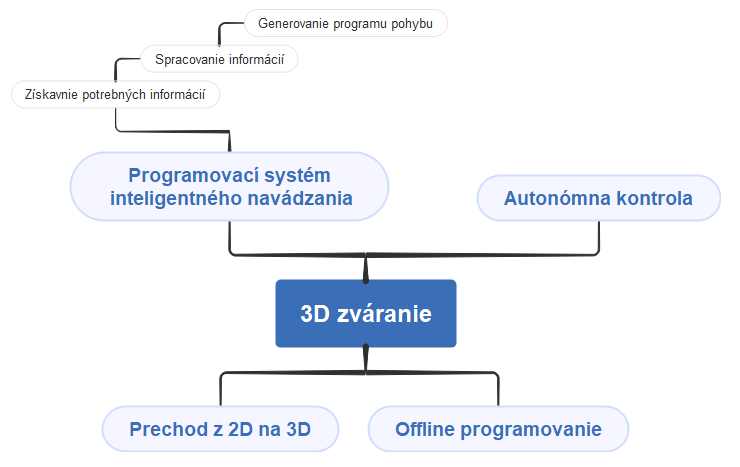
\includegraphics{myšlienková_mapa3.png}}
\label{fig}
\end{figure}

V myšlienkovej mape môžeme vidieť sekcie, ktorým sa bude článok venovať. Prvou sekciou bude Prechod z 2D na 3D (čast ~\ref{2dto3d}), kde bude opísaná problematika operácií v trojrozmernom priestore. V sekcii Offline programovanie (časť ~\ref{off}) sa budeme venovať ako toto programovanie funguje, porovnáme jeho výhody a nevýhody a porovnáme ho s umelou inteligenciou. Programovací systém inteligentého navádzania (časť ~\ref{AIsys})\cite{hlavny_zdroj} pozostáva z podsekcií, v ktorých sa budem venovať získavaniu informácií, ich spracovaniu a následne generovaniu programu pohybu. V tejto sekcii a daných podsekciách bude opísaný princíp automatizácie a perspektíva používania umelej inteligencie do budúcnosti. Po exekúcii programu je následne potrebná kontrola kvality vykonaných operácií, ktorým sa bude venovať sekcia Autonómna kontrola\cite{hlavny_zdroj} (časť ~\ref{AIcheck}).

\newpage
\section{Prechod z 2D na 3D} \label{2dto3d} %3

V súčasnosti väčšina robotov a strojov funguje na princípe offline programovania (viď ~\ref{off}), teda "klasickým" spôsobom - programátorom dopredu vytvorený program je spustený a robot alebo stroj dané kroky vykoná. Takto to funguje pri 2D a aj 3D formáte, akurát s tým rozdielom, že pri 3D je program zložitejší a ťažší na exekúciu. Samotný prechod by nebol až taký náročný, problém však nastáva, pokiaľ chceme implementovať umelú inteligenciu na zabezpečenie tohoto procesu, pretože učenie umelej inteligencie sa uskutočňuje priamo v procese.\cite{hlavny_zdroj}  To znamená, že umelá inteligencia sa učí rozoznávať, kedy spravila operáciu dobre a kedy nie. Tento proces je veľmi náročný vo viacerých sférach, no vyzdvihol by som najmä tieto - čas, finančná náročnost a v neposlednom rade zručnosť programátorov.

\section{Offline programovanie} \label{off} %4

Využíva sa najmä v robotickom výskume, inými slovami to môžeme nazvať i simuláciou. Ide o uistenie sa, že program vykonáva všetky operácie korektne ešte pred spustením na reálnom robotovi, aby sa predišlo zbytočným škodám. Niektoré simulátory dokonca umožňujú zadanie CAD modelu a systém automaticky vygeneruje trajektórie robota (viď ~\ref{AIsys:getinfo}), čo môže ešte viac zvýšiť efektivitu programovania.\cite{hlavny_zdroj} \newline

Výhody:
\begin{itemize}
\item Zníženie prestojov potrebných na programovanie robota, nakoľko robot musí byť zastavený iba počas sťahovania a testovania nového programu. 
\item Jednoduché testovanie mnohých rôznych prístupov k rovnakému problému, čo by bolo pre online programovacie metódy neefektívne.
\end{itemize}

Nevýhody:
\begin{itemize}
\item Virtuálne modely (pravdepodobne) nikdy nebudú schopné reprezentovať skutočný svet so 100\% presnosťou. Po aplikovaní programu na skutočného robota môže byť potrebné zmeniť programy.
\item Hoci offline programovanie znižuje prestoje robota, na druhej strane niekto musí venovať viac času vývoju simulácie, ako aj jej testovaniu na robotovi. 
\end{itemize}

\cite{off_pros_cons}

\section{Programovací systém inteligentného navádzania} \label{AIsys} %5 tu bude dosť textu

\cite{hlavny_zdroj}

\subsection{Získavanie potrebných informácií} \label{AIsys:getinfo} %5.1

Skenovanie zváracích dielov je nevyhnutnou podmienkou pre inteligentné programovanie zváracieho robota. Senzorom sa meria povrch zvaru a následne sa získavajú príslušné údaje potrebné na ďalšie vyhodnotenie. ~\cite{hlavny_zdroj} Existujú dve metódy skenovania: jednou je "manual teaching scanning", druhou je skenovanie extrahovaním dráhy skenovania z 3D modelu zváraných dielov. Prvá metóda je väčšinou realizovaná pomocou pevného počiatočného bodu, orientácie, intervalu skenovania a časov skenovania. Hoci táto metóda nemôže priamo naučiť trajektóriu skenovania, tak je jednoduchá a pohodlná na ovládanie. Druhá metóda využíva SolidWorks (softvér na premietanie 3D dielov a simulácie) pre sekundárny vývoj a na realizáciu extrakcie bodov z dráhy skenovania 3D modelu dielov. Následne podľa extrahovanej dráhy navádza robota pri skenovaní. Táto metóda je vhodná najmä pri skenovaní komplexnejších a zložitejších tvarov. ~\cite{hlavny_zdroj}

\subsection{Spracovanie informácií} \label{AIsys:processinfo} %5.2	

\subsection{Generovanie programu pohybu} \label{AIsys:movement} %5.3

\section{Autonómna kontrola} \label{AIcheck} %6 tu bude vela textu

\cite{hlavny_zdroj}

\section{Záver} \label{zaver} %7

Niečo zmysluplné, sumarizácia článku.

\newpage
\bibliography{literatura}
\bibliographystyle{plain} 
\end{document}
